\documentclass[dvipsnames]{article}
\usepackage[utf8]{inputenc}
\usepackage[english]{babel}
\usepackage[doublespacing]{setspace}
\usepackage[mathlines]{lineno}
\usepackage{minted}
\usepackage{numprint}
\usepackage{csquotes,xpatch}
\usepackage{fancyhdr,lipsum}
\usepackage{amsmath}
\usepackage{amsfonts}
\usepackage[normalem]{ulem}
\usepackage[color=blue!30!white,textsize=small,textwidth=30mm]{todonotes}
\usepackage[left=2cm,top=2cm,right=3.5cm,bottom=2cm,bindingoffset=0.5cm]{geometry}
\usepackage{bm}
%\linenumbers
\pagenumbering{arabic}

\usepackage{tabularray}
\usepackage{codehigh}
\UseTblrLibrary{booktabs}
\UseTblrLibrary{siunitx}
\newcommand{\tinytableTabularrayUnderline}[1]{\underline{#1}}
\newcommand{\tinytableTabularrayStrikeout}[1]{\sout{#1}}
\NewTableCommand{\tinytableDefineColor}[3]{\definecolor{#1}{#2}{#3}}


%TC:incbib

%%%%% For title page:
\usepackage{authblk}
\title{Title: something about recombination, genomic prediction and fitness}
\author[1,2,*]{Kenneth Aase}
\author[...]{...}
\author[2,3]{Henrik Jensen}
\author[1,2]{Stefanie Muff}
\author[4]{Susan Johnston}
\affil[1]{Department of Mathematical Sciences, Norwegian University of Science and Technology, Trondheim, Norway}
\affil[2]{The Gjærevoll Centre, Norwegian University of Science and Technology, Trondheim, Norway}
\affil[3]{Department of Biology, Norwegian University of Science and Technology, Trondheim, Norway}
\affil[4]{Edin, Edin, Edin}
\affil[*]{Corresponding author: Kenneth Aase, kenneth.aase@ntnu.no}
\date{}

%%%%% Running headline:
\renewcommand\rightmark{Short Title here}

%%%%% Bibliography
\usepackage{natbib}
\newcommand*{\citef}[1]{\footnote{\cite{#1}}}
%\usepackage[
%backend=biber,
%style=chicago-authordate,
%citestyle=authoryear,
%maxnames = 2,
%date=long,
%useprefix=true,
%sortlocale=norwegian,
%dateabbrev=false
%uniquename=false
%]{biblatex}

%\usepackage[style=authoryear, backend=biber, bibencoding=inputenc]{biblatex}
%\addbibresource{mylib.bib}
%\uspunctuation

%%%% Custom commands
\newcommand{\E}{\mathsf{E}}
\newcommand{\Prob}{\mathsf{P}}
\newcommand{\Var}{\mathsf{Var}}
\newcommand{\Cov}{\mathsf{Cov}}
\newcommand{\Corr}{\mathsf{Corr}}
\newcommand\given[1][]{\:#1\vert\:}
\newcommand{\N}[2]{\mathsf{N}\left(#1, #2\right)}
\newcommand*\diff{\mathop{}\!\mathrm{d}}
\newcommand{\ie}{\emph{i.e.}}
\newcommand{\eg}{\emph{e.g.}}
\newcommand{\Ie}{\emph{I.e.}}
\newcommand{\Eg}{\emph{E.g.}}
\newcommand{\note}[1]{\textcolor{red}{\scriptsize #1}}
\newcommand{\hl}{\textcolor{blue}}

% Table settings
\usepackage{booktabs}
\usepackage{multirow}
\usepackage{color, colortbl}
\newcommand{\ra}[1]{\renewcommand{\arraystretch}{#1}}
\definecolor{DarkGray}{gray}{0.8}
\definecolor{LightGray}{gray}{0.925}

% For figures and tables

\usepackage{graphicx}
\usepackage{cprotect}
\usepackage{float}
\floatstyle{plain}
\restylefloat{figure}
\floatstyle{plaintop}
\restylefloat{table}

\usepackage{caption} 
%\captionsetup[table]{skip=pt}

\usepackage[pdftex,bookmarks=true,hidelinks]{hyperref}
\hypersetup{
    %colorlinks=true,
    linkcolor=blue
}

% \renewcommand{\thetable}{S\arabic{table}}
% \renewcommand{\thefigure}{S\arabic{figure}}

\usepackage{verbatim}

\newcommand{\detailtexcount}[1]{%
  \immediate\write18{texcount -merge -sum -q #1.tex output.bbl > #1.wcdetail }%
  \verbatiminput{#1.wcdetail}%
}

\newcommand{\quickwordcount}[1]{%
  \immediate\write18{texcount -1 -sum -merge -q #1.tex output.bbl > #1-words.sum }%
  \input{#1-words.sum} words%
}

\newcommand{\quickcharcount}[1]{%
  \immediate\write18{texcount -1 -sum -merge -char -q #1.tex output.bbl > #1-chars.sum }%
  \input{#1-chars.sum} characters (not including spaces)%
}
\begin{document}

%%%% Comment in/out different .tex files to compile/include them or not

%TC:ignore
\maketitle
\newpage

\subsection*{ESEB Abstract}

\subsubsection*{Background}
Meiotic recombination during gamete formation is a fundamental evolutionary process. It is required to ensure proper chromosome segregation and promotes genetic diversity by shuffling alleles into novel haplotypes. This can create beneficial allele combinations and break up linkage between beneficial and harmful alleles, thereby facilitating adaptive evolution. However, high recombination rates also carry risks, such as introducing mutations at crossover sites, and potentially disrupting favorable allele combinations. Thus, recombination rates could affect individual fitness in opposite directions, suggesting a complex relationship with individual fitness.

Investigating the impact of recombination rates on fitness is complicated by the fact that identifying crossover positions during meiosis - and thus finding the crossover count - is only possible for individuals with genotyped offspring. This introduces a sampling bias which prevents measuring the recombination rates of individuals that are reproductively unsuccessful, excluding them from potential fitness analyses. Failure to account for these unmeasured individuals could potentially bias analyses of the fitness effects of recombination rates.

\subsubsection*{Materials and methods}
We used a long-term house sparrow study system from northern Norway with extensive pedigree, genotype, and fitness data to investigate the relationship between individual recombination rates and fitness components. The genomic and pedigree data were leveraged to measure autosomal crossover count (ACC) in adult house sparrows, resulting in one ACC measure per genotyped parent-offspring pair. We estimated sex-specific individual breeding values for ACC by using the phenotypic ACC measures for each parent as responses in a genomic prediction model. The genomic prediction, implemented as a Bayesian G-BLUP model, allowed us to estimate these breeding values in more than 2,600 phenotyped individuals, as well as in more than 2,900 additional individuals with no recorded offspring, correcting the aforementioned sampling bias and increasing the sample size of the subsequent fitness analyses.

We then related the estimated breeding values to sex-specific fitness components, including annual reproductive success and annual survival. As the individuals without ACC measurements had higher uncertainty in their estimated breeding values, we used measurement error modelling to account for the heterogeneous breeding value uncertainties. 

\subsubsection*{Results}
We found that individual ACC was related to male and female annual survival, with predicted annual survival peaking at intermediate breeding values for individual ACC. We also found weak evidence that males with intermediate breeding values had higher annual recruit production, but no evidence of a relationship with reproductive success in females. Altogether these results suggest potential stabilizing selection against extreme values of ACC, especially in male house sparrows.

\subsubsection*{Conclusions}
We demonstrate that individual variation in recombination rates influences fitness in a wild house sparrow population, with evidence of stabilizing selection on ACC particularly in male house sparrows. To interpret this association, we consider possible underlying biological mechanisms. On the methodological side, we present genomic prediction as a tool to address sampling biases. This novel approach allowed us to investigate the fitness consequences of a trait that can only be directly measured in reproductively successful individuals and allowed us to include several thousand individuals in the analysis that would otherwise have been excluded.

\section*{Introduction}

Rationale and background - Susan


% \begin{itemize}
%     \item 



    
% \end{itemize}

\section*{Methods}

\subsection*{House sparrow dataset}
% THIS IS AN ALMOST DIRECT LIFTOVER FROM THE MBE PAPER

All data in this study was collected from a meta-population of house sparrows inhabiting an 18-island archipelago off the Helgeland coast in Northern Norway (midpoint of 66$^\circ$32`N, 12$^\circ$32`E and covering 1600km\textsuperscript{2}). This metapopulation has been subject to an individual-based long-term study since 1993 \citep{Jensen2004-wt}. Birds are routinely captured and individually marked from the beginning of May to the middle of August and for approximately one month in the autumn using mist nets (adults and fledged juveniles), or as fledglings in accessible nests during the breeding season. A small (25 $\mu$ l) blood sample is collected from the brachial vein for DNA from every captured bird. Individual hatch year was determined as either (a) the first year recorded for nestlings or fledged juveniles captured in the summer and autumn, or (b) the year prior to first year recorded for birds first captured as female adults before June 1 or as males before August 1, or (c) a range including the year first recorded and the year prior for birds first captured as adult females after June 1 or adult males after August 1; hatch island is also recorded alongside hatch year \citep{ranke2021spatial, Saatoglu2021-ya}. Sampling was conducted in strict accordance with permits from the Norwegian Food Safety Authority and the Ringing Centre at Stavanger Museum, Norway.


\subsection*{Data}

\subsection*{Genomic Prediction}

Given measurements of the crossover count $y_{ij}$ of individual $i$ (estimated from offspring $j$) we model
\begin{equation*}
    y_{ij} = \alpha + \beta_\text{coverage} \cdot \text{coverage}_{ij} + g_i + \text{hy}_i + \text{hi}_i + \text{id}_i + \varepsilon_{ij}
\end{equation*}

Although the crossover count $y_{ij}$ is a count we treat it as a continuous Gaussian

priors on random effects: $PC(var = \hat{\sigma}^2_y / 2, 0.05)$ 

Fitting the GP model results in marginal posterior distributions for each breeding value. All of which approximately normal (can show by looking at QQ plots), so we can write
\begin{equation*}
    g_i \sim N(\mu_i, \sigma_i^2)
\end{equation*}

\subsection*{Fitness analyses}

We investigate the impact of the breeding values for sex-specific breeding values on fitness components.

% Sentences Susan asked for:
The Bayesian genomic prediction model gives us a full posterior for each individual breeding value $g_i$. 
In the fitness models, we can therefore incorporate the measurement error in these breeding value by sampling breeding values from these posterior distributions. 
Rather than treating the breeding values as having fixed, known values, we sample each breeding value $g_i$ in each MCMC iteration, and regress on these samples (and their square) in the logistic regression. 
(This is equivalent to assuming a Berkson measurement error model for the 
breeding values.)

\clearpage
List of models, in simple terms
\begin{itemize}
    \item Genomic prediction models (all on the following form): \begin{itemize}
        \item Likelihood: Gaussian
        \item Response: sex-specific crossover count
        \item Fixed effects: Total coverage
        \item Random effects: Breeding value, hatch year, hatch island, identity
    \end{itemize}
    \item Sex-specific adult ARS vs own breeding value for sex-specific crossover count \begin{itemize}
        \item Likelihood: zero-inflated poisson
        \item Response: annual reproductive success
        \item Fixed effects: \begin{itemize}
            \item intercept
            \item age and age squared (actually polynomial using bases for age, but don't worry about that)
            \item breeding value and breeding value squared (with measurement error model based on the uncertainty from the genomic prediction model)
            \item inbreeding coefficient
        \end{itemize} 
        \item Random effects: \begin{itemize}
            \item hatch year, 
            \item island (last recorded)
            \item identity
        \end{itemize}
        \item All fixed and random effects are used in both the zero-inflation component and the count component of the model
    \end{itemize}
    \item Sex-specific adult annual survival vs own breeding value for sex-specific crossover count \begin{itemize}
        \item Likelihood: binomial, with logit link
        \item Response: annual survival
        \item Fixed effects: \begin{itemize}
            \item intercept
            \item age and age squared (actually polynomial using bases for age, but don't worry about that)
            \item breeding value and breeding value squared (with measurement error model based on the uncertainty from the genomic prediction model)
            \item inbreeding coefficient
        \end{itemize} 
        \item Random effects: \begin{itemize}
            \item hatch year, 
            \item island (last recorded)
            \item identity
        \end{itemize}
    \end{itemize}
    \item Sex-specific adult ARS vs parental breeding value for sex-specific crossover count \begin{itemize}
        \item Identical to adult ARS model, except we use the breeding value for the parent of the same sex, and not the own breeding value. Same goes for inbreeding coefficient: we use the coefficient of the parent of the same sex, and not own fitness coefficient
    \end{itemize}
    \item Sex-specific adult annual survival vs parental breeding value for sex-specific crossover count \begin{itemize}
        \item Identical to adult survival model, except we use the breeding value for the parent of the same sex, and not the own breeding value. Same goes for inbreeding coefficient: we use the coefficient of the parent of the same sex, and not own fitness coefficient
    \end{itemize}
    \item Nestling recruitment (survival) vs parental breeding value for sex-specific crossover count \begin{itemize}
        \item Likelihood: binomial, with logit link
        \item Response: recruitment
        \item Fixed effects: \begin{itemize}
            \item intercept
            \item breeding value and breeding value squared (with measurement error model based on the uncertainty from the genomic prediction model)
            \item parental inbreeding coefficient
        \end{itemize} 
        \item Random effects: \begin{itemize}
            \item hatch year, 
            \item hatch island
            \item identity
        \end{itemize}
    \end{itemize}
\end{itemize}
\clearpage

\subsubsection*{Annual survival}

For individual $i$ in year $j$ we model the survival as a logistic GLMM, written here as a Bayesian hierarchical model:
\begin{align*}
    &g_i \sim N(\mu_i, \sigma_i^2) \\
    &\eta_{ij} = \alpha + \beta_g \cdot g_i + beta_{g^2} \cdot g_i^2 + \beta_\text{age} \cdot \text{age} + \beta_{\text{age}^2} \cdot \text{age}^2 + \beta_f \cdot f + \text{isl}_i + \text{year}_j + \text{id}_i + \varepsilon_{ij}\\
    &P(\text{survival}_{ij} = 1) = \text{logit}^{-1}(\eta_{ij})
\end{align*}


\subsubsection*{Annual reproductive success}

\section*{Results}

\begin{figure}
    \centering
    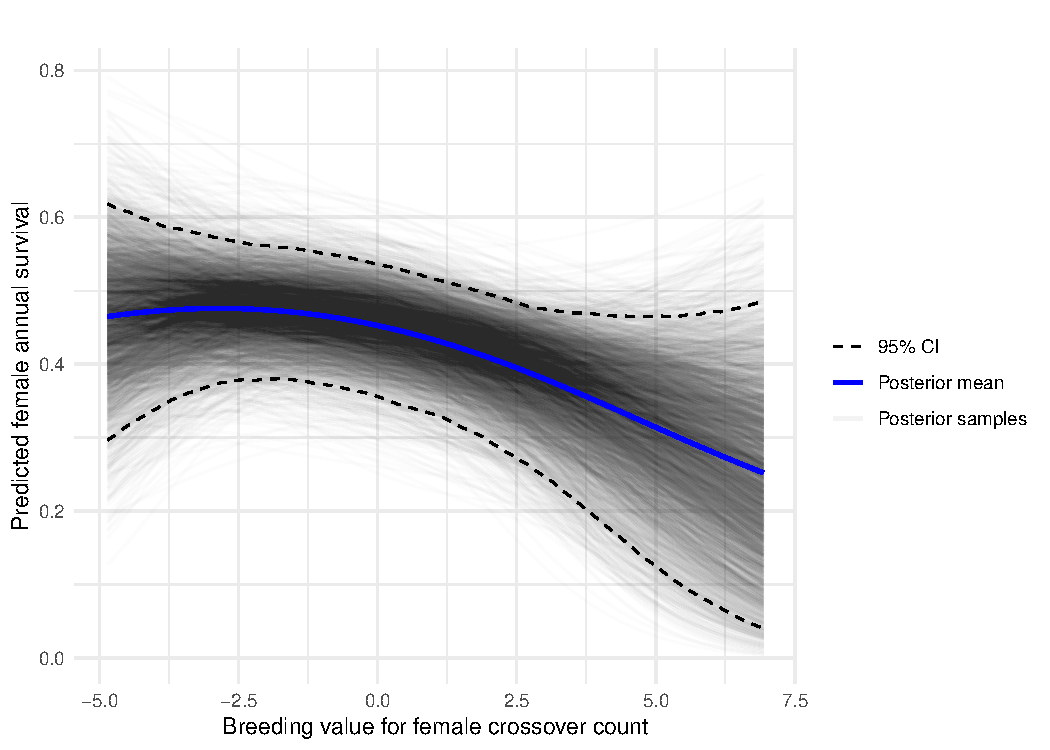
\includegraphics[width=0.91\linewidth]{figs/surv_bv_pred_f.pdf}
    \caption{...}
    \label{fig-surv_bv_f}
\end{figure}

\begin{figure}
    \centering
    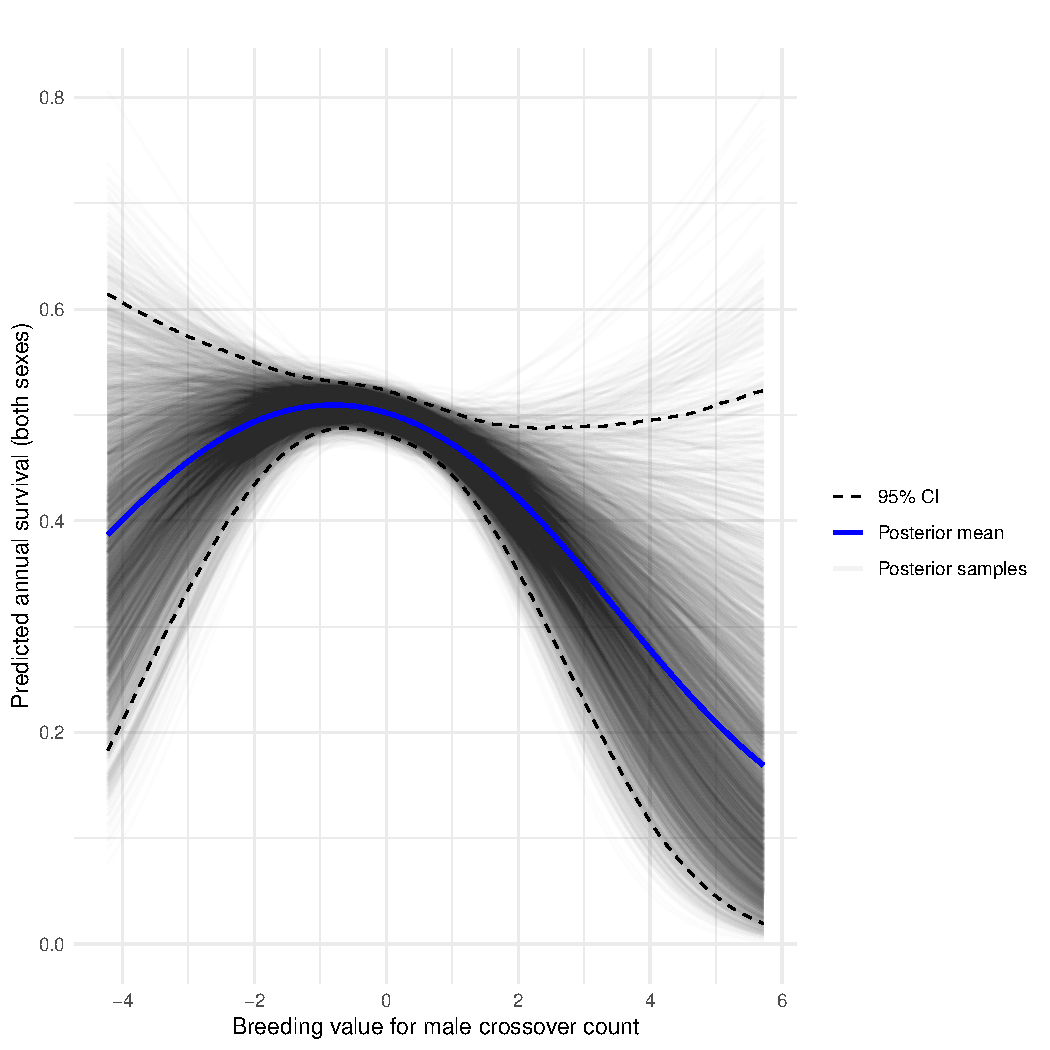
\includegraphics[width=0.91\linewidth]{figs/surv_bv_pred_m.pdf}
    \caption{...}
    \label{fig-surv_bv_m}
\end{figure}

\begin{figure}
    \centering
    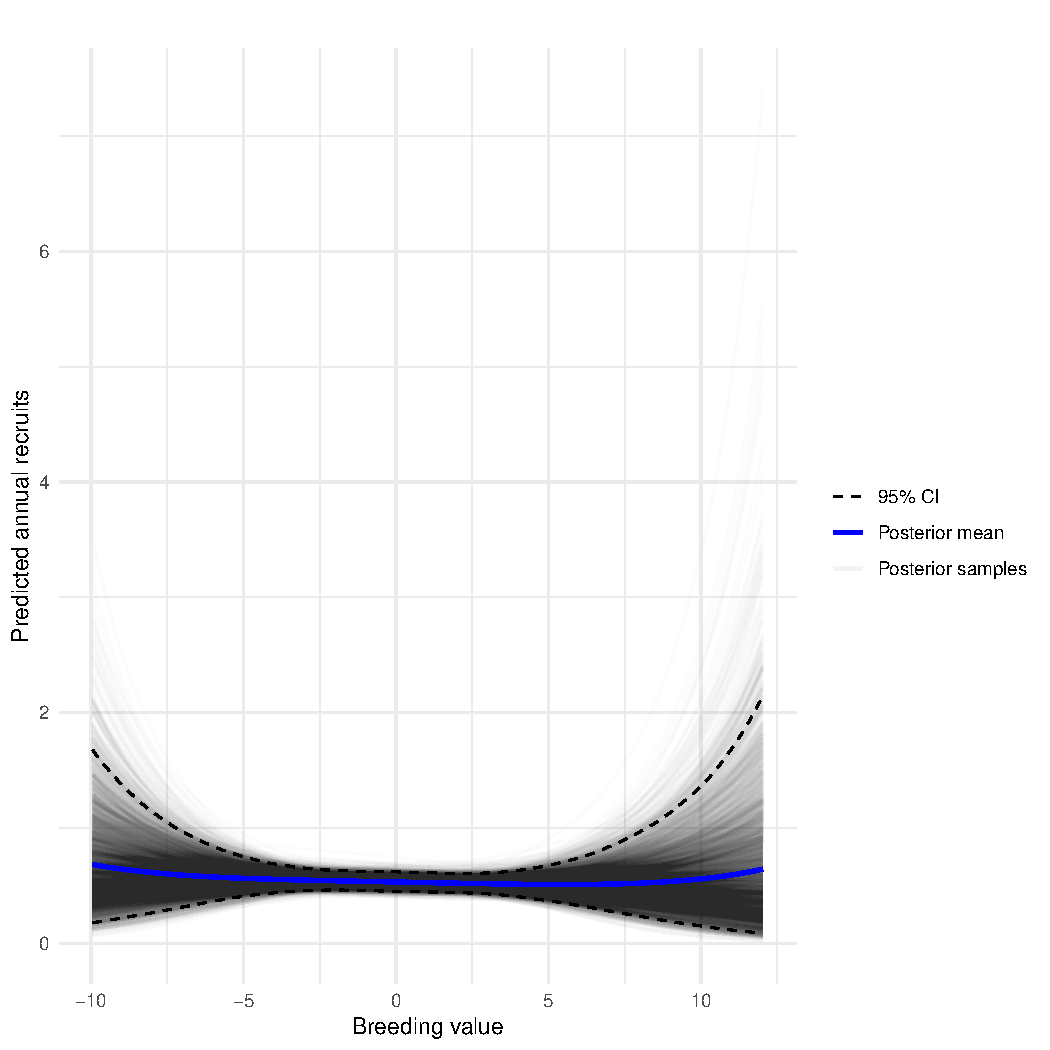
\includegraphics[width=0.91\linewidth]{figs/ars_bv_pred_f.pdf}
    \caption{...}
    \label{fig-ars_bv_f}
\end{figure}

\begin{figure}
    \centering
    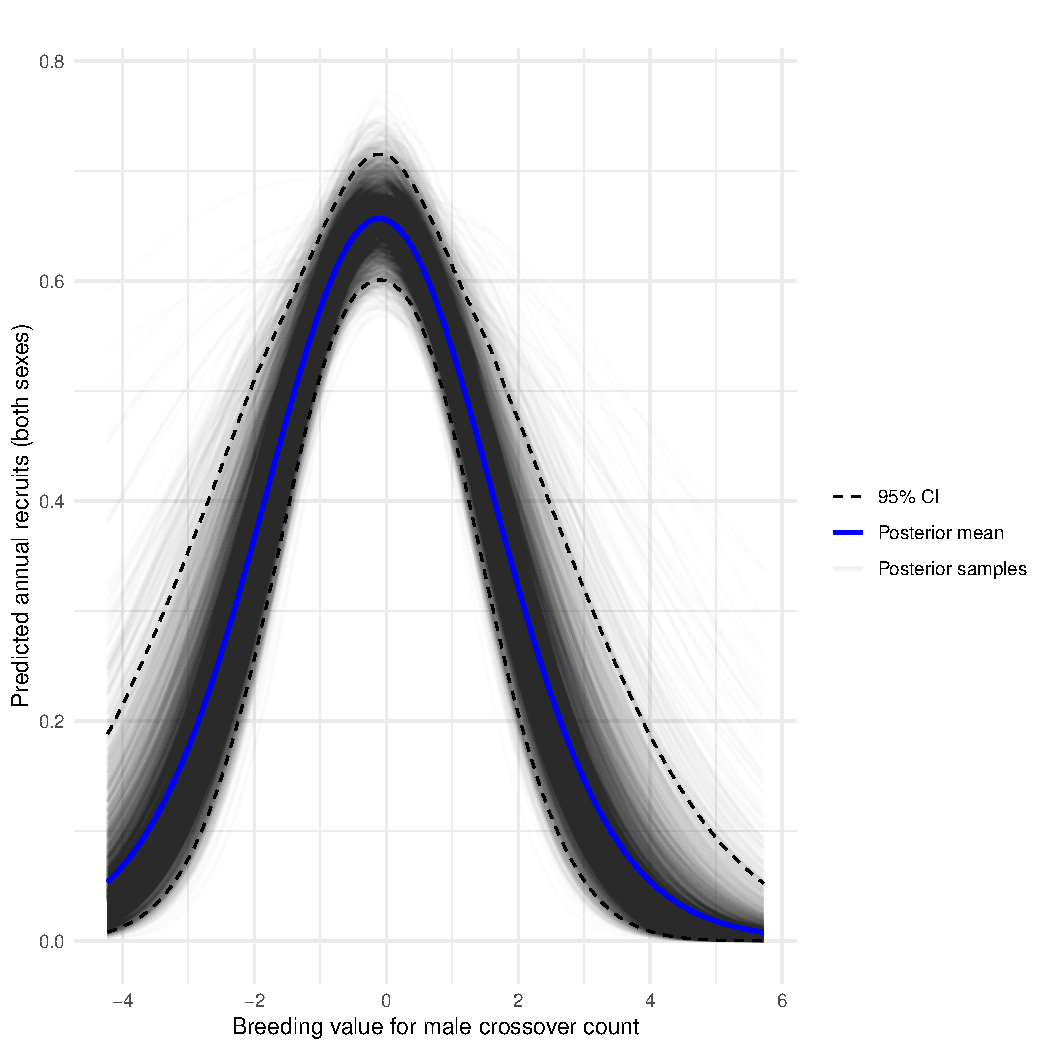
\includegraphics[width=0.91\linewidth]{figs/ars_bv_pred_m.pdf}
    \caption{...}
    \label{fig-ars_bv_m}
\end{figure}

\section*{Discussion}

\clearpage
\bibliographystyle{mee.bst}
\bibliography{mylib.bib}

\clearpage

\end{document}